\section{Appendix}

\section{Thief Scheduler}
\label{appendix:scheduler}
\romil{Move to rest of the paper}
\begin{table}[t!]
\footnotesize
\begin{tabular}{cl}
{\bf Notation} & {\bf Description}\\\hline
$\mathcal{V}$ & Set of video streams\\
$v$ & A video stream ($v \in \mathcal{V}$)\\\hline
$T$ & A retraining window with duration $\lVert T \rVert$ \\\hline
%$t$ & A point in time within a retraining window\\\hline
$\Gamma$ & Set of all retraining configurations\\
$\gamma$ & A retraining configuration ($\gamma \in \Gamma$)\\\hline
$\Lambda$ & Set of all inference configurations\\
$\lambda$ & An inference configuration ($\lambda \in \Lambda$)\\\hline
$\mathcal{G}$ & Total number of GPUs\\
$\delta$ & The unit for GPU resource allocation \\\hline
%$\Theta$ & The set of all possible GPU allocations  \\
%      & $\Theta = \{0, 1, ..., \frac{\mathcal{G}}{\delta}\}$\\
%$\mathcal{R}$ & The number of GPU resource unit $\delta$\\ 
%         & allocated for retraining ($\mathcal{R} \in \Theta$)\\
%$\mathcal{I}$ & The number of GPU resource unit $\delta$\\ 
%         & allocated for inference ($\mathcal{I} \in \Theta$)\\\hline
%$M_{v}^t$ & Set of all DNN instances for video $v$ at window $t$\\
%$m_{v\gamma}^t$ & A DNN instance based on $\gamma$ for video $v$ at $t$\\
%$\hat{m}_{v\gamma}^t$ & A \emph{retrained} DNN instance based on $\gamma$ for $v$ at $t$\\\hline
%$C^R(v, t, \gamma)$ & Retraining cost using $v$ and $\gamma$ at window $t$ \\
%$C^I(v, t, \gamma, \lambda)$ & Inference cost using $v$, $\gamma$, $\lambda$ at window $t$ \\
$A_T(v, \gamma, \lambda, \mathcal{R}, \mathcal{I} )$ & Inference accuracy for video $v$ for\\%at retraining \\
                                   %& window $T$ 
                                   &given configurations and allocations\\% given retraining configuration $\gamma$ \\
                                   %& inference configuration $\lambda$, $\mathcal{R}\delta$ GPUs for\\
                                   %& retraining, and $\mathcal{I}\delta$ GPUs for inference \\
$C_T(v, \gamma, \lambda)$ & Compute cost in GPU-time for video $v$ for\\%at retraining \\
                                   %& window $T$ for 
                                   &given configurations and allocations\\\hline%, given retraining configuration $\gamma$ \\
                                   %& and inference configuration $\lambda$ \\\hline
%$r_{vt\gamma g}$ & A binary variable indicates the system retrains \\
%& a DNN based on $\gamma$ for video $v$ at $t$ on GPU $g$\\\hline
$\phi_{v\gamma\lambda\mathcal{R}\mathcal{I}}$ & A set of binary variables ($\phi_{v\gamma\lambda\mathcal{R}\mathcal{I}}\in\{0,1\}$). \\
& $\phi_{v\gamma\lambda\mathcal{R}\mathcal{I}} = 1$ iff we use retraining config $\gamma$, \\
%& configuration $\gamma$, 
&inference config $\lambda$, $\mathcal{R}\delta$ GPUs for retraining,\\
& $\mathcal{I}\delta$ GPUs for inference for video $v$\\\hline
\end{tabular}
\caption{\label{tab:notations}Notations used in {\name}'s description.}\vspace{-12pt}
\end{table}

\subsection{Complexity Analysis.}
\label{complexity-analysis}
\emph{Assuming} all the $A_T(v, \gamma, \lambda, \mathcal{R}, \mathcal{I})$ values are known, the above optimization problem can be reduced to a multi-dimensional binary knapsack problem, a NP-hard problem \cite{DBLP:journals/mor/MagazineC84}. 
Specifically, the optimization problem is to pick binary options ($\phi_{v\gamma\lambda\mathcal{R}\mathcal{I}}$) to maximize overall accuracy while satisfying two capacity constraints (the first and second constraints in Eq~\ref{eqn:optimization}). %\ \forall v \in \mathcal{V}, \forall \gamma \in \Gamma, \forall \lambda \in \Lambda$ in a given window $T$.  
%Specifically, the optimization problem is to maximize accuracy (i.e., value of an item) by making binary decisions ($\phi_{v\gamma\lambda\mathcal{R}\mathcal{I}}$) in the system decision space (i.e., whether putting an item in a knapsack or not). 
%It is multidimensional because the decisions need to satisfy two constraints (the first and second constraints in Eq~\ref{eqn:optimization}).
%It is multi-choice because the system can only make one decision for each video (the third constraint in Eq~\ref{eqn:optimization}). 
%Hence, even when assuming that we know all the $A_T(v, \gamma, \lambda, \mathcal{R}, \mathcal{I})$ values, the problem is a multi-choice, multidimensional binary knapsack problem, which is known to be NP-hard \cite{DBLP:journals/mor/MagazineC84}. 
In practice, however, getting all the $A_T(v, \gamma, \lambda, \mathcal{R}, \mathcal{I})$ is \emph{infeasible} 
%because this requires we actually train the edge DNN $\forall \gamma\in\Gamma, \forall v \in \mathcal{V}$ and run inference with all the retrained DNNs as well as the non-retrained DNNs $\forall v \in \mathcal{V}, \forall \lambda \in \Lambda$. 
because this requires training the edge DNN using all retraining configurations and running inference using all the retrained DNNs with all possible GPU allocations and inference configurations.%, for all the video streams.
%In fact, doing so completely defeats the purpose of the resource optimization problem. 

The uncertainty of $A_T(v, \gamma, \lambda, \mathcal{R}, \mathcal{I})$ resembles the multi-armed bandits (MAB) problem \cite{robbins1952some} to maximize the expected rewards given a limited number of trials for a set of options.
%chooses among a set of options using trials, and by observing the reward at the end of each trial. %choosing among a set of slot machines at each round of play, and upon that selection observing a reward realization. 
%The player aims to maximize the expected rewards given a limited number of trials. 
%Because of data shift, the past experience on rewards ($A(v, T, \gamma, \lambda)$) can change significantly among different window, which means the underlying rewards are non-stationary and the optimal strategy is intractable without limiting the variation of rewards \cite{DBLP:conf/nips/GurZB14}. 
Our optimization problem is more challenging than MAB for two reasons.
%First, the cost of each trial ($C_T(v, \gamma, \lambda)$) varies significantly unlike the MAB problem where the cost of each trial is fixed.
First, unlike the MAB problem, the cost of trials ($C_T(v, \gamma, \lambda)$) varies significantly, and the optimal solution may need to choose cheaper yet less rewarding options to maximize the overall accuracy.
%Thus, the optimal solution may leverage cheaper yet less rewarding option to maximize the overall accuracy, instead of looking for the highest reward option. %which is unlike the MAB problem. 
%Second, since we are optimizing for multiple players simultaneously using the same set of resources, the optimal solution may leverage cheaper yet less rewarding option to maximize the overall accuracy, which is unlike the MAB problem. 
%As discussed above, it is a NP-hard multiple knapsack problem even if all the rewards are known. 
%This is fundamentally different from the MAB problem, whose goal is to find and leverage the maximum rewarding option as often as possible because the cost of pulling each arm is fixed. 
Second, getting the reward $A_T(v, \gamma, \lambda, \mathcal{R}, \mathcal{I})$ after each trial %is too expensive because this 
requires "ground truth" labels that are obtained using the large golden model, which can only be used judiciously on resource-scarce edges (\S\ref{subsec:continuous}).
%. As \S\ref{subsec:continuous} discussed, we have to be judicious about running the golden model on resource-constrained edges. 


In summary, our optimization problem is computationally more complex than two fundamentally challenging problems (multi-dimensional knapsack and multi-armed bandits).  
%Thus, we proceed to design an efficient approximate heuristic. 

% PickConfigurations
% For the given allocation, finds the best configuration and returns the accuracy gotten by the best configuration and given resource allocation.

\begin{algorithm}[t]
\small
 \KwData{Resource allocations in {temp\_alloc[]}, configurations ($\Gamma$ and $\Lambda$), retraining window $T$, videos $V$}
 \KwResult{Chosen configs $\forall v \in V$, %for the given $\mathcal{R}^\prime$ and $\mathcal{I}^\prime$, 
 average accuracy over $T$}
 
     chosen\_accuracies[] $\leftarrow$\{\}; chosen\_configs[] $\leftarrow$\{\}\;
     \For{\text{\em v} in $V$\text{\em []}}{
        %\tcc{Pick highest accuracy inference cfg}
        infer\_config\_pool[] = $\Lambda$.{\bf where}(\text{resource\_cost} < temp\_alloc[v.inference\_job] \&\& accuracy $\geq a_\text{MIN}$ )\;
        % Add alpha min filter in cfg_pool
        infer\_config = {\bf max}(infer\_config\_pool, {\bf key}=accuracy)\;
        %\tcc{Pick training configuration}
        best\_accuracy = 0\;
        % best\_training\_cfg = None\;
        \For{\text{\em train\_config} in \text{\em $\Gamma$}}{
            \tcc{Estimate accuracy of inference/training config pair over retraining window} % Done using profiles.
            accuracy = {\sf\footnotesize EstimateAccuracy}(train\_config, infer\_config, temp\_alloc[v.training\_job], $T$)\;
            \If{\text{\em accuracy} > \text{\em best\_accuracy}} {
                best\_accuracy = accuracy\;
                best\_train\_config = train\_config\;
            }
        }
        chosen\_accuracies[v] = best\_accuracy\;
        chosen\_configs[v] = \{infer\_config, best\_train\_config\}\;
     }
    {\bf return} chosen\_configs[], {\bf mean}(chosen\_accuracies[])\;
 
 \caption{\bf\small PickConfigs}
 \label{algo:pickconfigs}
\end{algorithm}
% \revtext{
% \section{Retraining window sensitivity analysis}
% \begin{figure} [t!]
%  	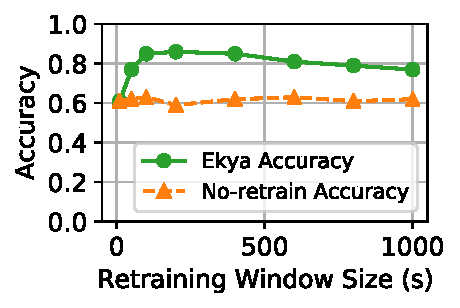
\includegraphics[width=0.9\linewidth]{results/sensitivity/retraining_window_sensitivity.pdf}
% 	\caption{\small \bf A sensitivity analysis of the retraining window parameter. \name is robust to a wide range of retraining window values and gracefully degrades to an accuracy equivalent of no retraining if the window size is too small. If the window size is too large, the model's generalizability becomes the limiting factor, slowly reducing the accuracy as more training data accumulates.
% 	}
% 	\label{fig:window-sensititvity}
% \end{figure}

% A key parameter in \name is the a retraining window parameter which governs how frequently a model will be retrained. In each retraining window, data samples are accumulated and then used to retrain the model for the subsequent window. The size of this window is set by the retraining window parameter. To evaluate the sensitivity of \name to the retraining window parameter, we evaluate \name's performance on the cityscapes dataset with 2 GPUs and 4 streams and vary the window sizes. We compare the accuracy achieved by \name across different retraining window sizes, ranging from 10 seconds to 1000 seconds. As a baseline, we also compare a no-retraining baseline where a pre-trained model is used without any continous retraining.

% As is seen in Figure~\ref{fig:window-sensititvity}, Ekya is robust to reasonable choices of retraining window sizes. When the retraining window size is too small (10 seconds), the accuracy of \name is equivalent to no retraining accuracy simply because there is insufficient time and resources to perform any retraining. As the retraining window increases (>10 seconds), \name's performance quickly ramps up to because the thief scheduler is able to allocate resources to retraining. As the retraining window size further increases (>400 seconds) Ekya's performance slowly starts degrading because of the inherently poor generalizability of compressed models \S\ref{subsec:continuous-measurement}. However, this degradation is a function of the choice of compressed model and can be avoided by using a different compressed model or choosing a better retraining window. 
% }